%!TEX program = xelatex
\documentclass[cn,11pt,chinese]{elegantbook}

\title{算法导论全作业集合}
\subtitle{2020Autumn - Introduction to Algorithm-homework}

\author{jzpa}
\institute{USTC}
\date{\today }
\version{1.0}
\bioinfo{声明}{不保证质量与正确性,仅供学习交流}

\extrainfo{Victory won\rq t come to us unless we go to it. --- M. Moore}

\logo{logo-blue.png}
\cover{cover.jpg}

% 本文档命令
\usepackage{array}
\newcommand{\ccr}[1]{\makecell{{\color{#1}\rule{1cm}{1cm}}}}
% 修改目录深度
\setcounter{tocdepth}{2}

\begin{document}

\maketitle
\frontmatter

\chapter*{写在前面的话}
\markboth{Introduction}{前言}

算法是一门很重要的课。
与我预先基于自己浅薄知识所做的设想不同的是,这门课所教授的并不是有关算法如何产生的大一统理论,
而是如何分析、运用、理解一些经典的结论和算法。
所谓大一统的计算理论,在目前依然是一个遥不可及的梦想。

此处记录了我在2020秋季学期算法导论课的所有作业的答案。
作业的题目请移步\href{http://202.38.86.171/}{课程主页}查看(仅校内学生可以访问)。
当然,此处需要再次声明

\begin{center}
  请妥善使用。由于传播或使用本文档所导致的一切问题,本人拒不负责。
\end{center}

\underline{有空可能会补上原题}

\vskip 1.5cm

\begin{flushright}
jzpa\\
\today 
\end{flushright}

\tableofcontents
%\listofchanges

\mainmatter

%\chapter{前言}

%注意保护眼睛

\chapter{Algorithm Homework 1}

\section{查找问题}

\subsection{(a)线性查找伪代码与正确性证明}

伪代码如下
\begin{lstlisting}[language = C++]
int LinearSearch(A,v)
    int i
    n = A.length
    for i=1 to n do
        if(v == A[i])
            return i;
        i = i + 1;
    return NIL
\end{lstlisting}


  使用循环不变式证明这一算法的正确性 \\\textcircled{1} \textbf{初始化:}$i=1$的时候,在$i=2$之前,这个算法已经完成了对$A[1]$到$A[i-1]$(事实上就是没有元素的空集)的查找,
  如果$v$存在于这些数组元素之间,就已经直接返回下标$i$值(空集中显然不存在元素,所以未发生操作),并且函数结束,所以不会轮到$i=1$。
\\\textcircled{2} \textbf{保持:}假设完成$i=j$的时候满足循环不变式,那么这个算法已经完成了对$A[1]$到$A[j-1]$的查找,
  如果已经查到了$v$,那么应该早就已经返回下标i并且函数结束。对于进入下一次迭代,函数体检查$A[j]$的值,如果$A[j]==v$,那么会直接返回$j$而跳出循环结束函数,保证了在下一次循环$i=j+1$的时候依然能满足循环不变式。
\\\textcircled{3} \textbf{终止:}导致循环终止的条件是$i>n$或者在这之前已经发现满足条件的$i$而跳出循环,
  如果是后者,根据循环不变式,显然算法完成了它的任务找到了满足条件的$i$并范围
  如果是前者,根据循环不变式,数组本身的大小就是$n$,所以算法已经查找完了整个数组内所有的元素而都没有发现满足条件的$A[i]==v$,
      所以$v$不在$A$中出现,直接返回$NIL$,满足算法设计要求
\\综上,这个算法正确

\subsection{(b)计算复杂度}

答:记检查次数为$X$,平均需要检查次数为$EX = \Sigma_1^n kP(X = k) = \Sigma_1^n k/n = \Theta(n/2) = \Theta(n)$\\
    而最坏情况下,也就是$v$不存在于数组内的情况下,最多需要检查$n=\Theta(n)$次

\section{判断相关等式和陈述}

答:理由采用简述
\begin{itemize}
  \item a)错误,可以举出反例$f(n) = 1/n$,该情况下等式右侧是$\mathrm{O} (1/n^2)$,显然两边不等 
  \item b)正确,由于$f(n)$,$g(n)$都是非负渐进函数,在$n$足够大的情况下,显然$max(f(n),g(n)) \le f(n)+g(n) \le 2*max(f(n),g(n))$
  \item c)正确,由于$f(n)$,$g(n)$都是非负渐进函数,而且在$n$足够大的情况下,存在$k'$使得$f(n) \ge k'*\mathrm{O} (f(n)) $,于是在$n$足够大的情况下,$f(n) \le f(n) + \mathrm{O} (f(n)) \le 1/k' * f(n)$
  \item d)错误,可以举出反例$f(n) = g(n) =n$,显然$f(n) = \Omega (g(n))$但$f(n) \neq  \mathrm{o}(g(n))$
\end{itemize}

\section{证明等式}

先证明第一个结论

  显然有$n$足够大时
  \begin{equation}
      \begin{aligned}
          lgn! &= lg1+lg2+lg3+\dots + lgn \\
                &\le \underbrace{lgn+lgn+\dots +lgn}_{n\mbox{个}} \\
                &= nlgn
      \end{aligned}
  \end{equation}
  又因为$n$足够大时,$\sqrt{n} \le n/2$,所以
  \begin{equation}
    \begin{aligned}
        1/4nlgn &= 1/2nlg\sqrt{n} \\
                &\le \underbrace{lg\sqrt{n}+lg\sqrt{n}+\dots +lg\sqrt{n}}_{[n/2]+1\mbox{个}} \\
                &\le \underbrace{lg([n/2])+lg([n/2]+1)+\dots +lgn}_{[n/2]+1\mbox{个}}\\
                &\le lg1+lg2+lg3+\dots +lgn
    \end{aligned}
  \end{equation}
  所以有$n$足够大时,$1/4nlgn \le lgn! \le nlgn$,所以$lgn! = \Theta (nlgn)$

下证第二处结论

  显然有$n$足够大时,满足如下式子
  \begin{equation}
    \begin{aligned}
        0\le \frac{2^n}{n!} &= \frac{2^n}{1*2*3*4*\dots *n}\\ 
                         &=\frac{3^2}{2} *\frac{2^n}{3*3*3*4*5*6*\dots *n}\\
                         &\le \frac{3^2}{2} *\frac{2^n}{3^n} 
    \end{aligned}
  \end{equation}
  由于
  $$\lim_{n\rightarrow \infty} \frac{3^2}{2} *\frac{2^n}{3^n} = 0$$
  所以可证得
  $$\lim_{n\rightarrow \infty} \frac{2^n}{n!} = 0$$
  所以有
  $$n! = \omega (2^n)$$
  同时,
  \begin{equation}
    \begin{aligned}
        0\le \frac{n!}{n^n} &= \frac{1}{n} * \frac{2}{n} * \frac{3}{n} * \dots * \frac{n}{n} \\ 
                          &\le \frac{1}{n}
    \end{aligned}
  \end{equation}
  由于
  $$\lim_{n\rightarrow \infty} \frac{1}{n} = 0$$
  所以可证得
  $$\lim_{n\rightarrow \infty} \frac{n!}{n^n} = 0$$
  所以有
  $$n^n = \mathrm{o} (n!)$$

\section{代入法证明}

  使用代入法证明\\
  \textcircled{1} 设$T(1) = \Theta (1)$\\
  \textcircled{2} 根据递归式有,假设$T(n) = \mathrm{O}(lgn)$对$1$到$(n-1)$都成立,那么当$n$足够大时有
  \begin{equation}
    \begin{aligned}
        T(n) &= T([n/2]) + 1 \\
              &\le T(n/2) + 1 \\
              &\le clg(n/2) + 1 \\
              &= clgn -clg2 +1 \\
              &\le (c+10)lgn
    \end{aligned}
  \end{equation}
  所以$T(n)$仍满足递归假设\\
  综合\textcircled{1} \textcircled{2}有,
  $$T(n) = \mathrm{O} (lgn)$$

\section{递归树法}

递归树生成过程如下
\begin{lstlisting}
  T(n)

  cn
  |
  |---------|
  |         |
  T(n-a)   T(a)
  
  cn
  |
  |------------|
  |            |
  c(n-a)       T(a)
  |
  |---------|
  |         |
  T(n-2a)   T(a)
  
  ......  
\end{lstlisting}
每层和分别为$cn,c(n-a)+T(a),c(n-2a)+T(a),\dots$,求和得解为$\Theta (n^2)$

\section{主方法解递归式}

\subsection{$T(n) = 2T(n/4)+\sqrt{n}$的情况}
  解:使用主方法解\\
  首先可以看到这个递归式满足形如$T(n) = aT(n/b) + f(n)$的情况,且$a=2 \ge 1,b=4 > 1,f(n) = \sqrt{n}$,可以使用主方法先行分析\\
  那么有$n^{log_b a} = n^{log_4 2} = n^{1/2} = \Theta (f(n))$,所以有
  $$T(n) = \Theta (\sqrt{n}lgn)$$

\subsection{$T(n) = 2T(n/4)+n^2$的情况}
  解:使用主方法解\\
  首先可以看到这个递归式满足形如$T(n) = aT(n/b) + f(n)$的情况,且$a=2 \ge 1,b=4 > 1,f(n) = n^2$,可以使用主方法先行分析\\
  那么有$\exists \epsilon = 1/2 > 0,s.t. n^{log_b a +\epsilon } = n^{log_4 2+1/2} = n,f(n) = n^2 = \Omega (n)$,所以有
  $$T(n) = \Theta (n^2)$$

\section{主方法讨论}

答:根据书本原文上对于主方法的初步定义,这是不可以的。但是根据本课程所讲授的扩展后的主方法可以解决这个问题。

理由(为什么书本上初步定义的主方法不适用):尽管其算式形式满足形如$T(n) = aT(n/b) + f(n)$的情况,且$a=4 \ge 1,b=2 > 1,f(n) = n^2lgn$,
    但是比较发现,$f(n)=n^2lgn$与$n^{log_b a} = n^{log_2 4} = n^2$之间不仅显然不满足第一、二类判断条件,
    同时这两者尽管有$n^2lgn$渐近大于$n^2$的情况, 但并不是多项式意义上的大于,
    对任意正常数$\epsilon$,比值$f(n)/n^{log_b a}$都渐近小于$n^{\epsilon}$,
    因此,递归式落入了第二、三类条件之间的间隙。

理由(补充):但实际上,本课程授课时曾给出一个更新后的扩展的主方法,其中第二种情况扩展为$f(n) = \Theta (n^{log_b a} lg^k n)$,
            这样一来,这个式子就刚好符合$k=1$的情况,而对应也能得到$T(n) = \Theta (n^2 lg^2 n)$

计算上界:使用代入法证明,证得其一个上界为$\mathrm{O} (n^2lgn)$

  使用代入法证明\\
  \textcircled{1} 设$T(1) = \Theta (1)$\\
  \textcircled{2} 根据递归式有,假设$T(n) = \mathrm{O}(n^2lgn)$对$1$到$(n-1)$都成立,那么当$n$足够大时有
  \begin{equation}
    \begin{aligned}
        0\le T(n) &= 4T(n/2) + n^2lgn \\
                  &\le 4c*(n/2)^2lg(n/2) + n^2lgn \\
                  &= cn^2lg(n/2) + n^2lgn \\
                  &= (c+1)n^2lgn-cn^2lg2 \\
                  &\le (c+1)n^2lgn
    \end{aligned}
  \end{equation}
  所以$T(n)$仍满足递归假设\\
  综合\textcircled{1} \textcircled{2}有,
  $$T(n) = \mathrm{O} (n^2lgn)$$

\chapter{Algorithm Homework 2}

\section{堆排序复杂度分析}

堆排序可以分为初始化堆和调整堆两部分,那么首先看初始化堆

对于都按升序排列的情况,那么在初始化时对于每一个非叶子结点,都需要进行调整,把它与孩子结点进行比较和交换,使得以这个非叶子结点为根的子树是一个堆(假设在它后面的结点都已经经过这个调整了)。

考虑到初始的数组就是按升序排列的,从底层往高层开始执行初始化堆的操作,一开始,任一非叶子结点都没被操作过,且显然小于它的子树里所有的元素。若操作进行到某一个阶段,假设所有没被操作过的结点都小于它的子树的所有元素,
那么考察某个处于第i层第k个并且尚未被操作的结点x,在这之后紧接着的一次比较和交换操作只可能发生在i+1层往下和第i层位置大于等于k的结点,
假如发生在第i+1层的结点,若该结点不属于x的子树,那么这个操作并不影响x与其子树间的大小关系,对于第i层位置大于k的结点,同样他们及其子树的元素与x的子树无关,故操作后也不影响x小于其子树的元素
若该结点属于x的子树,由于x本身就比子树中所有元素都小,该操作后x依然小于子树中所有元素,如果操作发生这个结点在第i层第k个,即恰为x,那么该轮操作后x就不是“未被操作的结点”了。
所以综上归纳得到这个过程中,任何一个非叶子结点在被操作前都小于其所有的子树元素,那么轮到每个结点的操作需要的交换次数约为$(k-i)$次,所以有
$$\sum\limits_{i=1}^{k-1} (k-i)*2^{i-1} = 2^k-k+1 \approx  n-logn+1 = \varTheta (n)$$
而对于按降序排列的情况,那么在初始化时直接不用进行调整,通常算法只需要验证得到所有的值符合条件即可,而不需要进行后续交换,那么显然其时间复杂度就是$O (n)$

对于后面的调整堆部分,两种情况下都需要每次用最后一个结点替换掉堆顶再进行调整,设最后一个结点的序号是$m$,那么有
$$\sum\limits_{m=1}^{n-1}logm = log(n-1)! = O (nlogn)$$
综合两个过程,结果均为 $O (nlogn)$

\section{快速排序}

\subsection{叶结点深度相关证明:}

首先要看到递归树的主要形态,由于$T(n) = T(\alpha n)+T((1-\alpha )n)+f(n)$它在每一个非叶子结点$T(m)$分支为$T(\alpha m)$和$T((1-\alpha )m)$两棵子树,直到$m\thickapprox 1$(m小于一个足够小的常量)时才停止生长成为叶子结点。
那么假如某个结点的高度是$i$,显然其展开两个孩子结点或者作为叶子结点前满足式子
$$T(m) = T(\alpha ^{r1} (1-\alpha )^{r2} n),r1+r2 = i-1$$
$\because 0< \alpha \le \frac{1}{2} $,且如果是叶子结点,$m \approx 1$,那么在这一前提下

若$r1+r2 = (r1+r2)_{min}$,有$r2=0$,故
$$1\approx m = \alpha ^{r1} (1-\alpha )^{0} n = \alpha^{r1+r2} n$$
$$(r1+r2)_{min} = \frac{-lgn}{lg\alpha } $$
即递归树叶子结点的最小深度

同理有$r1+r2 = (r1+r2)_{max}$时,$r1=0$,故
$$1\approx m = \alpha ^{0} (1-\alpha )^{r2} n = (1-\alpha )^{r1+r2} n$$
$$(r1+r2)_{max} = \frac{-lgn}{lg(1-\alpha )} $$

\subsection{证明平衡划分的概率}

在快速排序里,我们的目的是找到数组中的一个成员,并且基于数组中各元素与它的比较关系,将数组划分为两份部分。

不妨忽视舍入问题,考虑到这是一个随机数组,我们通过快速排序的算法会找到一个作为划分基准点的关键元素,通常情况下,不妨设我们每次选取数组中的第一个元素为关键元素。

假如我将拿到的数组进行递增的排序成一个新数组再去考察,那么显然,其中的每一个元素都有同样的概率在排序前出现在原数组中的第一个而被算法选中,即,新数组中每一个位置所对应的元素等可能地是关键元素。

设新数组的长度为L,关键元素在其中的位置是$a$,那么$[0,a]|[a,L]$就是PARTITION产生基于关键元素的划分,
假如$a\in [0,\alpha L] \cup [L-\alpha L ,L]$,那么这个产生的划分$[0,a]|[a,L]$是比$[0,\alpha L]|[\alpha L,L]$更加不平衡的,反之要想比其更平衡,a应当落在$[\alpha L,L-\alpha L]$之间,由前面的讨论,其概率为

$$\frac{(L-\alpha L) - \alpha L}{L} = 1-2\alpha $$

\chapter{Algorithm Homework 3}

\section{排序算法稳定性分析}

插入排序、归并排序、计数排序都是稳定的算法,而快速排序、堆排序都是不稳定的算法。

方法:为每个数据增加一个序数域,里面存储着原数组中该数据元素的位置,
然后对于任何一个排序算法,其比较规则在原有的比较规则作为优先的情况下,若判定为相等,就继续比较序数域的值来判定比较结果。
根据这一新的比较规则,将不存在两元素相等的情况,原有的相同元素必将因为序数域的值被区分开来,在排序后依然维持原有序数的大小关系,故称稳定排序

开销:设规模为n,空间开销将在原有的基础上增加$\varTheta (n)$,
时间开销上仅仅是在原有比较的基础上增加了一层判断,
相当于所有的比较操作时间乘以一个常数,
所以时间复杂度前后均等于属于同一个$\varTheta (f(n))$,
记原比较次数为$m$,那么额外时间开销就是$\varTheta (m)$。

\section{RANDOM-SELECT最坏情况}

9、8、7、6、5、4、3、2、1

\section{证明基于比较的排序算法的最坏情况耗时}

证明:由于给定的n个数的序列是完全随机的,也就是说它可能是这n个数$n!$种排列里的任意一种,
同理由对称性,给定n个数的任意排列都有可能是需要的排序序列,
那么作为一个可行的排序算法,不论其具体实现如何,其输入的序列如何,
其比较树的叶子结点就应该覆盖到这n个数所有的排列,
即该树的叶子结点数应当$\ge n!$。而众所周知,假如一棵二叉树的高度是$H$,
那么其叶子结点最多的情况就是这棵树是完全二叉树的情况,设叶子结点数为$k$
即
$$2^{H-1}\ge k$$
所以有
$$2^{H-1}\ge n!$$
此处的H反映的其实就是时间开销,即时间开销$T = \varTheta (H)$,可知其为
$$H =\varOmega (log(n!))$$
又因为
$$log(n!) = \varTheta  nlogn$$
所以最终得到
$$T = \varOmega (nlogn)$$
所以任何基于比较的算法从n个元素的任意序列中构造一棵二叉搜索树,其最坏情况下需要$\varOmega (nlogn)$的时间

\section{证明k次连续后继查找所需的时间}
首先这是k次连续的查找,那么假设第一个查找结点为S,最后一个查找结点为T。

如果S和T属于同一路径,即其中一者为另一者的祖先,
那么这个过程就相当于对一个以其中祖先结点为根结点的子树进行的遍历操作,
显然其时间复杂度为$O (k)$

如果S和T不属于同一路径,那么取两者最近的共同祖先V,路径必然要经过V。
该过程显然可以看作从S到V和从V到T两个过程之和,考察S到V过程,其时间顶多是$O (2n)$,
V到T同理,于是总时间就是$O (2n) + O (2n) = O (n)$

综合起来时间复杂度就是$O (n+k)$

\chapter{Algorithm Homework 4}

\section{红黑树操作}

\subsection{插入操作}
在依次插入41、38、31、12、19、8之后最终的红黑树如图\ref{Ch4S1_1}
\begin{figure}[htbp]
	\centering
	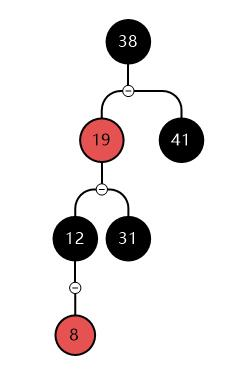
\includegraphics[width=0.3\textwidth]{image/Ch4S1_1.jpg}
	\caption{红黑树插入最终图}
  \label{Ch4S1_1}
\end{figure}

\subsection{删除操作}
在依次删除8、12、19之后分别对应的红黑树如图\ref{Ch4S1_2}
\begin{figure}[htbp]
	\centering
	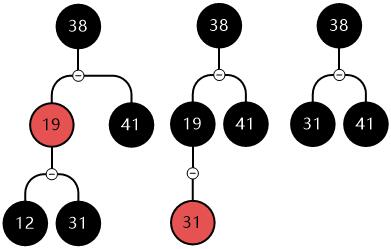
\includegraphics[width=0.6\textwidth]{image/Ch4S1_2.jpg}
	\caption{红黑树删除逐步图}
  \label{Ch4S1_2}
\end{figure}

\section{区间重叠点分析}

\subsection{重叠点包含某区间端点}

证明如下。

首先设区间集合为${I_i}$,且共有$n$个集合,而重叠点为集合$S$,那么由定义显然有
\begin{equation}
    S = \bigcap _{i=0}^n I_i \nonumber
\end{equation}
显然S不可能是无限的,其必然具有上界或者下界,不妨假设其有一个上界,由确界原理可知其有上确界,记为$\alpha $。

$\alpha $为上确界,具有两种可能,一种是$\alpha $在S中是孤立点,考察一系列区间从左到右运算取并集,要想产生孤立点,要么存在一个仅包含一个孤立点的区间,这种情况下结论显然成立,假如没有这样的区间,那么在逐个合并过程中,理应在某个时刻,出现诸如$\dots ,b]\cap [b,\dots $的操作,其中左侧是进行到该操作之前前面所有已计算过的集合的并集,后侧是这之后的第一个集合。那么这个问题可以化归到讨论$\alpha $不是孤立点的情况。

统一讨论另一种可能,即$\alpha $不是孤立点的情况,即$\exists \epsilon_0 > 0,\quad s.t. (\alpha - \epsilon_0,\alpha ) \subseteq S $,由于$S$是所有区间的并集,所以有
\begin{equation}
    \forall x \in (\alpha - \epsilon_0 ,\alpha) ,\quad x \in I_i,\quad i=1,2,3,\dots  \nonumber
\end{equation}
但是,同样有
\begin{equation}
    \forall x \in (\alpha ,\alpha + \epsilon_0 ) ,\quad x \notin S  \nonumber
\end{equation}
由S为所有区间的并集,有
\begin{equation}
    \exists I_0 \in {I_i},\quad s.t.\forall x \in (\alpha ,\alpha + \epsilon_0 ) ,\quad \quad x \notin I_0 \nonumber
\end{equation}
那么对于该$I_0$而言,$\alpha $就是它的上端点。

证毕

\subsection{数据结构构建}

具体构建伪代码如下,默认忽略各边界条件:

\begin{lstlisting}[language = c++]
struct Mark{
	value;
	struct Mark* next;
}; 
struct Mark* CreateMarkList(){
	struct Mark* head;
	head=(struct Mark*)malloc(sizeof(struct Mark));
	head->value=0;
	head->next=NULL;
} 
int Insert(struct Mark* head, left, right){
	int Tag;
	struct Mark* p,*p_pre;
	struct Mark *Node,*NodeRight;
	p=head;
	p_pre=NULL;
	Tag=1; 
	while(p->next!=NULL ){
		p_pre=p;
		p=p->next;
		Tag=!Tag;
		if(p->value >= left) break;
	}
	if(Tag && (p_->value.rightEdge > left or equal and both close)){
		Node=(Mark *)malloc(sizeof(Mark));
		Node->value = left;
		p_pre->next = Node;
		Node->next=p;
		p=Node;
		head->value += 1;
	}
	else{
		p=p_pre;
	}
	Tag=!Tag;
	p_pre=p;
	while(p_pre->next!=NULL){
		p=p_pre->next;
		Tag=!Tag;
		if(p->value >= right) break;
		p_pre->next=p->next;
		free(p);
		head->value -= 1;			
	}	
	if(Tag && mirror case){
		Node=(Mark *)malloc(sizeof(Mark));
		Node->value = right;
		p_pre->next = Node;
		Node->next = p;	
		head->value += 1;
	}
	return(0);
} 
int Delete(struct Mark* head, left, right){
	int Tag;
	struct Mark* p,*p_pre;
	struct Mark *Node,*NodeRight; 
	p=head;
	p_pre=NULL;
	Tag=1; 
	while(p->next!=NULL ){
		p_pre=p;
		p=p->next;
		Tag=!Tag;
		if(p->value >= left) break;
	}
	if(!Tag && (p_->value.rightEdge > left or equal and both close)){
		Node=(Mark *)malloc(sizeof(Mark));
		Node->value = left;
		p_pre->next = Node;
		Node->next=p;
		p=Node;
		head->value += 1;
	}
	else{
		p=p_pre;
	} 
	Tag=!Tag;
	p_pre=p;
	while(p_pre->next!=NULL){
		p=p_pre->next;
		Tag=!Tag;
		if(p->value >= right) break;
		p_pre->next=p->next;
		free(p);
		head->value -= 1;			
	}	 
	if(!Tag && mirror case){
		Node=(Mark *)malloc(sizeof(Mark));
		Node->value = right;
		p_pre->next = Node;
		Node->next = p;	
		head->value += 1;
	}
	return(0);
} 
value find_pom(struct Mark* head){
	struct Mark* p;
	p=head;
	while(p->next!=NULL){
		p=p->next;
	}
	return p->value;	
}
\end{lstlisting}

\section{斐波那契堆的相关讨论}

\subsection{删除的另一种写法}
显然不是,这个过程需要对每一个孩子结点做一次cut操作,那么至少相当于$O$(最大degree),即应当作$O(D(n))$,即$O(lgn)$,不可能是常数时间复杂度。

\subsection{给出紧凑上界}
$O(x.degree+c)$

\chapter{Algorithm Homework 5}

\section{编写操作伪代码}

使用链表表示和加权合并启发式策略,写出MAKE-SET,FIND-SET和UNION操作的伪代码

\begin{lstlisting}[language = C++]
MAKE-SET(x){
	create S	
	x.prev = S
	x.next = null
	S.head = x
	S.tail = x
	S.rank = 1
}
FIND-SET(x){
	if x != x.prev
		return x.prev.head
	else
		return x
}
UNION(x,y){
	LINK(FIND-SET(x), FIND-SET(y))
}
LINK(S1,S2){
	if S1.rank < S2.rank
		S2.tail.next = S1.head
		S2.tail = S1.tail
		p = S1.head
		while p != null	
			p.prev = S1
			p = p.next
	else
		do the mirror work
}
\end{lstlisting}

\section{求解0-1背包问题}

代码如下
\begin{lstlisting}
maxValue(weight[], value[], W) {
	n = weight.length;
	if n == 0
		return 0;
	int[][] dp = new int[n][W];
	for k = 1 to W
		if k >= weight[1]
			dp[1][k] = value[1];
		else
			dp[1][k] = 0;
	}
	for i = 2 to n
		for k = 1 to W
			With_i = (k-weight[i] >= 0) ? (value[i] + dp[i][k-weight[i]]) : 0;
			Without_i = dp[i][k];
			dp[i][k] = max(With_i, Without_i);
		}
	}
	return dp[n][W];
}
\end{lstlisting}
实际上就是画了一张$n*W$的表格,除了第一列直接赋值,后面每一列都只需要参考与它本身操作线性的数据和时间来填写,所以最后耗时相当于O(表格的规模),即O(nW)

\chapter{Algorithm Homework 6}

\section{钢条切割扩展问题}

思路就是:相对于原版的算法,每次计算收益的时候额外把切割成本算进去,每次计算收益都有需要切割和不需要切割两种可能性分类。算法如下:
\begin{lstlisting}[language = c++]
EXTENDED-BUTTOM_UP-CUT-ROD(p,n)
	let r[0..n] and s[0..n] be new arrays
	r[0]=0
	for j = 1 to n
		q = p[j]
		s [j] = j
		for i = 1 to j-1
			if q < p[i] + r[j-i] - c
				q = p[i] + r[j-i] - c
				s[j] = i
		r[j] = q
	return r and s
\end{lstlisting}
如此r数组存储了各种长度钢条最佳切割时的收益,而s数组存储了最佳切割方案。输出最优切割方案的算法不变。

\section{计算有向无环图从s到t的最长加权简单路径}

思路就是,首先对有向无环图做拓扑排序,将顶点排作一列并以此顺序建立数组映射,随后对这个数组使用自底向上的动态规划法即可
为简化起见,拓扑排序部分的算法以及图的细节部分只做省略说明,算法如下
\begin{lstlisting}
TOPOLOGICAL-SORT(G)
1:	call DFS(G) to compute the degree_in for each vertex v
2:	if a vertex v0's degree_in is 0, insert it onto the tail of a linked list
3:	delete all the edge from v0 to other vertex
4:	turn to step 1, repeat 1-3 until all the vertexes have been insert into the linked list
5:	return the linked list
DAG-LONGEST_PATHS(G,weight,s,t)
	let n = the number of vertex	
	let v[1...n]  TOPOLOGICAL-SORT(G)
	locate the s,t in the r as si,ti
	let r[0...n] and s[0...n] be new arrays
	r[si] = 0
	q = -INFINITE
	for i = si+1 to ti
		for j = si to i-1
			if q < weight(v[j],v[i]) + r[j]
				q = weight(v[j],v[i]) + r[j]
				s[i] = v[j]
		r[i] = q
	return r and s
\end{lstlisting}
如此r[ti]保存了s到t的最大权重和,而s数组则存储了路径信息,打印输出的算法同钢条切割

\section{最优二叉树问题}

绘制表格如图\ref{Ch6S3_list}
\begin{figure}[htbp]
	\centering
	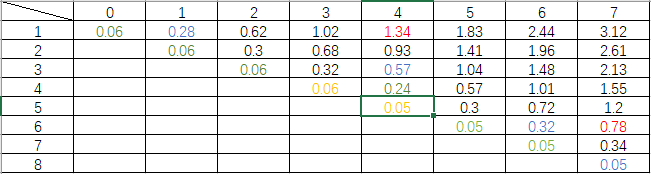
\includegraphics[width=\textwidth]{image/Ch6S3_list.png}
	\caption{求解最优二叉树表格}
  \label{Ch6S3_list}
\end{figure}

基于此绘制二叉树如图\ref{Ch6S3_map},菱形结点为叶子,圆形结点为非叶子结点,从左到右按照序号i排列
\begin{figure}[htbp]
	\centering
	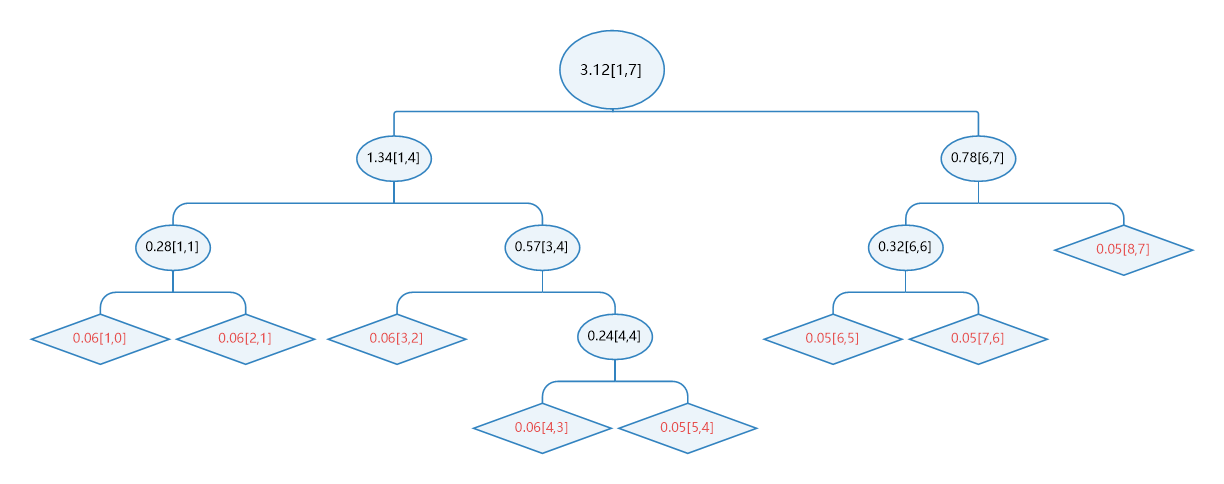
\includegraphics[width=\textwidth]{image/Ch6S3_map.png}
	\caption{求解最优二叉树图}
  \label{Ch6S3_map}
\end{figure}


\section{公司宴会交际问题}

思路阐述与计算复杂度分析:

本质上是递归算法,每次对于一个结点(上司)以及它的子树(下属),
维护两个属性,一个是上司出席时以该上司结点为根的子树所能具有的最大的交际评分和,记作v.a,
一个是上司不出席时该树的最大交际评分和,记作v.b,

对于叶结点,v.a即其交际评分,v.b取0,而对于非叶子结点,它的两个属性可作如下计算:
v.a = 其所有孩子的b属性之和
v.b = 其所有孩子的a、b属性最大值之和

在计算这两个属性的过程中,为了能够输出最佳方案对应的宾客名单,再对每一个结点额外维护一个switch属性,
该属性记录的是,当它的上司未被选中时,以它的上司为根结点的子树取到最大交际评分时该结点是否被选中,
如果被选中则记录1,反之记录0,
显然这个属性可以在计算a,b属性的同时进行维护,每个结点维护一次

最后最顶层上司结点a、b属性最大者即此次宴会最佳名单对应的交际评分和。

在输出最优解宾客名单时,对顶层上司开始自顶向下递归,分为两类:

一类递归:根结点参加与否完全自由的递归分析,
如果其a属性大于b属性,那么该上司加入宾客名单,
同时对所有该上司的孩子进行以该孩子不参加宴会为前提的进一步分析,即二类递归,
否则,上司不加入,对所有孩子执行一类递归

二类递归:根结点不参加的递归分析,
对所有孩子直接执行一类递归

计算属性本质上是做了一轮树的遍历,而自顶向下递归本质上也是做了一轮遍历,两轮遍历中对于每一个结点的操作显然都是常数时间,
所以设人员总数为$v$,实际计算复杂度是$\Theta(v)$

具体算法实现如下:
\begin{lstlisting}
CALCULATE(root,score)
	let n be the number of the vertexes
	let a[1..n], b[1..n], switch[1..n] be new arrays
	CALCULATE-AUX(root,score,a,b,switch)
	if a[root] < b[root]
		q = b[root]
	else
		q = a[root]
	return q and switch
CALCULATE-AUX(head,score,a,b,switch)
	if head = NULL
		return
	else
		a[head] = score[head];
		b[head] = 0;
		for (p = head.lchild ; p != NULL ; p = p.rbrother)
			CALCULATE-AUX(p,score,a,b,switch)
			a[head] += b[p]
			if a[p]>b[p]
				b[head] += a[p]
			else
				b[head] += b[p]
		if a[head] > b[head]
			switch[head] = 1
		else
			switch[head] = 0
PRINT(head,switch,pre_switch)
	if head = NULL
		return
	if pre_switch = 0
		head_switch = switch[head]
		if head_switch = 1
			print head
	else
		head_switch = 0
	for (p = head.lchild ; p != NULL ; p = p.rbrother)
		PRINT(p,switch,head_switch)
\end{lstlisting}

\section{覆盖点集的最小区间问题}

思路阐述和正确性分析:

本质上分3步

1.对所有点做一个排序,耗时$\Theta(nlogn)$;

2.从最小的点开始,以该点为起点构造一个长度为1的区间

3.从点集中删掉被包括在该区间内的点,返回重复第2步直到没有新的点为止,这些构造的区间集就是我们要的

首先假设一个最优解,其由若干区间构成,
那么由于其为最优解,最小的点必然包含在它最靠左的区间内,
假设最小点是$x_0$,这个区间为$[a,b]$,
如果这个点并不是区间的左端点,由于$x_0$本身是最小点,那么$[a,x_0)$本身应当不含任何点,
所以修改$[a,b]$为$[x_0,x_0+1]$的话,这个区间集也依然是最优解,也就是说贪心算法的第2步所探索的解依然属于最优解之一,
接下来分析递归部分,在这一修改过的最优解的基础上,从点集中取出包含在$[x_0,x_0+1]$的点,
那么由于其最优解的特性,若从点集中去掉这些点,同时从最优解中去掉$[x_0,x_0+1]$,其依然为修改后的点集的最优解,
这一点,证明贪心算法的第3步递归依然不会破坏探索到的解属于最优解之一的特性,
所以该算法最终找到的解依然是最优解

具体算法如下
\begin{lstlisting}
COVER-POINT(PointSet)
	let S be an empty set of intervals
	HEAP-SORT(PointSet)
	while PointSet is not empty
		min_tmp = MIN(PointSet)	
		add [min_tmp,min_tmp+1] to the S
		delete the point in [min_tmp,min_tmp+1] from PointSet
	return S
\end{lstlisting}

\section{找零问题}

思路阐述与正确性分析:

贪心算法,总是优先尝试用最大面值的硬币来找,找到可能的最大的硬币后,先把这枚硬币给顾客,再对剩下需要找的钱进行递归

对该算法正确性的分析,应当着眼于其递归的过程。每次算法找到当前需要找零数下能使用的最大的硬币,把它拿给顾客后再处理剩下需要找的钱,
这个过程本质上是把一个问题分割成了两个子问题,其中子问题A是一个等同于该硬币面值的找零问题,子问题B是一个等同于剩下钱数的找零问题,
而分割后的子问题AB中,显然A在算法里直接得到了最优解硬币数1,而假如B也找到了最优解,下面证明这两个子问题的最优解合起来是原问题的最优解,

首先由问题题意容易得出,找零问题需要找的零钱数越大,其需要使用的最少硬币数必然不小于零钱数更小的问题。基于这个原理,观察两个子问题,
如果原问题存在一个最优解,将其内部硬币按从大到小排序,其中面值最大的硬币$value_max$显然不可能超出子问题A的值$value_A$,
那么如果$value_max$ = $value_A$,那么显然该算法对于问题AB的划分包含了最优解,
如果$value_max < value_A$,那么基于$value_max$,最优解被分成了两个部分,其中一部分是$value_max$的一枚硬币,另一部分是剩下的硬币,
显然这两部分解分别是$value_max$的子找零问题C的最优解和总找零$-value_max$的子找零问题D的最优解,C解为1枚硬币,而D解硬币数不小于B解硬币数,
故可得知AB子问题合起来也必然是最优解之一,

如此一来,该贪心算法只要B子问题找得到最优解,那么算法本身必然找到的是最优解,由其递归性可知,B子问题的分割必然会在某一步变成单硬币的可解问题,
所以该贪心算法总是能找到最优解

具体算法实现如下:
\begin{lstlisting}
PAY-BACK(n)
	let s be an empty set
	while(n>0)	
		if n >= 25
			add 25 to s
			n -= 25
		else if n >= 10
			add 10 to s
			n -= 10
		else if n >= 5
			add 5 to s
			n -= 5
		else
			add 1 to s
			n -= 1
	return s
\end{lstlisting}

\chapter{Algorithm Homework 7}

\section{摊还分析}

\subsection{聚合法}
解:\\
设$C_i$表示第$i$个操作的代价,那么
\begin{equation}
	C_i = \left\{ 
		\begin{aligned}
			&i \quad,i\mbox{为2的某个幂} \\
			&1 \quad,\mbox{其它}
		\end{aligned}
    \right. \nonumber
\end{equation}
故$n$个操作总代价为
\begin{equation}
	\begin{aligned}
		\sum_{i=1}^n C_i&= n-\lfloor lgn\rfloor  +\sum_{j = 0}^{\lfloor lgn \rfloor } 2^j \\
						&\le n + \frac{1-2^{\lfloor lgn\rfloor +1}}{1-2} \\
						&\le n + (2n-1) \\
						&< 3n 
	\end{aligned} 
	\nonumber
\end{equation}
所以操作的摊还代价是$O (\sum C_i) / n = O (1)$

\subsection{核算法}
解: \\
操作代价同上,设摊还代价的某上限替代为
\begin{equation}
	\hat{C_i} = 3 \nonumber  
\end{equation}
若$i$为2的某个幂,则其少支付了$i-3$的代价\\
若$i$不为2的幂,那么其多支付了2代价\\
在$i$到达2的某个幂和下一个幂之间,设下一个幂的值为$i_0$,\\
在那之前恰多支付了$2(i_0/2-1)=i_0 -2$的代价,\\
所以$\sum \hat{C_i}\mbox{总是}\ge \sum C_i$

故得出摊还代价为$O (1)$

\subsection{势能法}
解: \\
状态用$i$来表征,令$i = 2^j + k$,其中$j$是使得$k \ge 0$的最大整数,那么,设势函数为
\begin{equation}
	\Phi (i) = 2k \nonumber
\end{equation}
由定义可知$\Phi (i) \ge 0$,所以这个势函数是合法的。\\
于是有
\begin{equation}
	\begin{aligned}
		\hat{C_i} &= C_i + \Phi (i) - \Phi (i-1) \\
				&\le 3
	\end{aligned}
	\nonumber
\end{equation}
所以摊还代价为$O(1)$

\section{d维离散傅里叶变换问题}

\subsection{证明可分解为一维问题}
证明: \\
在第一维度对于$k_1$值,有
\begin{equation}
	y_{k_1,k_2,\dots ,k_n} = \sum_{j_1=0}^{n_1-1} a_{j_1,k_2,\dots ,k_d} \omega_{n_1}^{j_1k_1} \nonumber
\end{equation}
故得,计算$n/n_1$个独立一维DFT
\begin{equation}
	y_{k_2,k_3,\dots ,k_d}= (y_{1,k_2,\dots ,k_d},y_{2,\dots },\dots ,y_{n_1-1,k_2,\dots ,k_d}) = DFT(a_{k_2,k_3,\dots ,k_d}) \nonumber
\end{equation}
以一维结果作为输入,计算第二维
\begin{equation}
	\begin{aligned}
		y_{k_1,k_2,\dots ,k_n} &= \sum_{j_2=0}^{n_2-1} (\sum_{j_1=0}^{n_1-1} a_{j_1,j_2,k_3,\dots ,k_d} \omega_{n_1}^{j_1k_1}) \omega_{n_2}^{j_2k_2} \\
							&= \sum_{j_1=0}^{n_1-1} \sum_{j_2=0}^{n_2-1} a_{j_1,j_2,k_3,\dots ,k_d} \omega_{n_1}^{j_1k_1} \omega_{n_2}^{j_2k_2} 
	\end{aligned}
	\nonumber
\end{equation}
故得,计算$n/n_2$个独立一维DFT
\begin{equation}
	y_{k_1,k_3,\dots ,k_d}= (y_{k_1,1,\dots ,k_d},y_{k_1,2,\dots },\dots ,y_{k_1,n_2-1,\dots ,k_d}) = DFT(y_{k_1,k_3,\dots ,k_d}) \nonumber
\end{equation}
以此类推直到第$d$维,有
\begin{equation}
	y_{k_1,k_2,\dots ,k_d}= \sum_{j_1=0}^{n_1-1} \sum_{j_2=0}^{n_2-1} \dots \sum_{j_d=0}^{n_d-1} a_{j_1,j_2,\dots ,j_{d-1}} \omega_{n_1}^{j_1k_1} \omega_{n_2}^{j_2k_2} \dots \omega_{n_d}^{j_dk_d} \nonumber
\end{equation}
故得,计算$n/n_d$个独立一维DFT
\begin{equation}
	y_{k_1,k_2,\dots ,k_{d-1}}= (y_{k_1,k_2,\dots ,k_{d-1},1},y_{k_1,k_2,\dots ,k_{d-1},2},\dots ,y_{k_1,k_2,\dots ,k_{d-1},n_d-1}) = DFT(y_{k_1,k_2,\dots ,k_{d-1}}) \nonumber
\end{equation}
证毕

\subsection{证明可交换性}
证明: \\
$\omega_{n_1}^{j_1k_1}$对于$k_1$共有$n_1$种取值,$\omega_{n_2}^{j_2k_2}$对于$k_2$共有$n_2$种取值,\dots \\
这个计算方法的实质,实际上是对这些取值做了$n_1n_2n_3\dots n_d = n$中全排列再进行求和,调整维度的顺序只是影响了求和次序,对于每个排列对应的值并无影响。 \\
所以维度次序的变换并不影响计算结果。证毕。

\subsection{证明时间复杂度}
证明: \\
直接求解其时间复杂度。第$i$维度需要计算$n/n_i$个独立一维DFT,而每个DFT的时间复杂度为$O(n_ilgn_i)$,故总时间复杂度为
\begin{equation}
	\begin{aligned}
		T(n) &= \sum_{i=1}^d \frac{n}{n_i}O(n_ilgn_i) \\
			&= \sum_{i=1}^d O(nlgn_i) \\
			&= O(nlg\prod_{i=1}^d n_i) \\
			&= O(nlgn)
	\end{aligned}
	\nonumber
\end{equation}
与d无关,证毕

\chapter{Algorithm Homework 8}

\section{欧拉回路}

\subsection{证明度数恒等式}
证明:

首先假设图G有一条欧拉回路,其包含了所有的边,那么以如下方法重新构造图$G=(V,E)$。

首先构造$|V|$个孤立点,
随后沿着欧拉回路一条条添加边,每添加一条边$e=(u,v)$,都意味着$u.out-degree+=1$,$v.in_degree+=1$,
且不造成其它的度数变化,由于这条边属于欧拉回路,那么
必$\exists e_u = (a,u)$,在这一次添加之前紧接着或者最后被添加,
其效果使得$u.in-degree+=1$且不造成$u$的其它度数变化,
也必$\exists e_v = (v,b)$,在这一次添加之前紧接着最先被添加,
其效果使得$v.out-degree+=1$且不造成$v$的其它度数变化。

即任一条边的添加带来的某点的出/入度增加,
必然会在其紧邻的某次添加或最后/最先一次添加(相当于第一次添加前面的紧邻/最后一次添加后面的紧邻)中被其带来的入/出度增加平衡,
所以到最后添加完毕,对任一点$v$,$in-degree(v) = out-degree(v)$

另外一方面,当图中任意点$v$都满足$in-degree(v) = out-degree(v)$时,可以由下面所给出的方法,构造出一条欧拉回路从而得证。
\begin{itemize}
	\item \textbf{第一步:}选定任意一个点$v_0$作为起点,标记$p\rightarrow v_0$,设已经找到的一部分欧拉回路为$S$,此时$S$为空集
	\item \textbf{第二步:}从p指向的点$u$的出边中选择一条未被走过的出边$(u,v)$,置$p = \rightarrow v$,标记该条边已经走过
	\item \textbf{第三步:}若p指向的点已经没有未被走完的出边,判断走过的边数,若已经走完全边,则算法停止走过的路径就是欧拉回路,
							若尚未走完全边,当S为空时,将找到的回路加入,若S不为空,由于这是一个强连通图,假设S中已经有一条回路,
							那么两条回路之间必然有交点,那么基于这个交点可以将两条回路合并为一条回路,更新S
\end{itemize}

首先,由于出入度相同,从$v_0$出发,每一次经过$v-0$只会等量增加其出入度,故若算法终止,最后也必然在$v_0$结束,形成环路。而且由第三步退出条件可以看出,
此时的回路已经经过了所有边,故只要算法停止,得到的必是合法的欧拉回路

其次,图的点数、边数有限,而算法每一轮必然会走过一条边,当走过$|V|$条边时必然结束,并且由于出入度相同,算法应当总是能找到一条未被走过的出边,直到构成回路,
然后再次从一个新的边开始,直到所有边都被遍历。故此,该算法必能在有限时间内停止得到结果。

\subsection{寻欧拉回路算法}

算法分析:

正确性已经在前面证得
\begin{itemize}
	\item \textbf{第一步:}只执行一次耗时$O(1)$
	\item \textbf{第二步:}执行最多$|E|$次,耗时$O(E)$
	\item \textbf{第三步:}执行次数最多$|E|$次,合并环路次数等于环路个数$-1$,采用合理的数据结构,每次合并的工作量加起来应当为$O(|E|)$
\end{itemize}

算法描述:
\begin{lstlisting}
FIND-EULER-ROUTE(G)
	choose a vertex ,let p points to it;
	visited[|E|]  = {0}; count = 0;
	create an empty link list S;
	visited[0] = 1;//points to the first edge not visited
	while count < |E|
		for each p's out edge e && visited[e] == 0
			add e to S
			visited[e] = 1
			visited[0] = next edge not visited
			break
		if no edge finded
			let p points to visited[0]'s edge's begin vertex
	print S;
\end{lstlisting}

\section{套利交易}
为方便起见ab一起实现,本质是Floyd-Warshall算法,其时间复杂度为$O(n^3)$,
附加一个矩阵用于存储最短路径信息便于输出,其附加的时间复杂度显然$O(n^3)$,
合计$O(n^3)$
打印部分就是单纯地利用矩阵里存储的路径信息依次查找打印即可,
每次递归的部分为$O(1)$,总时间复杂度$O(n)$
\begin{lstlisting}[language = c++]
FLOYD-WARSHALL(R)
n=R.rows
D(0)=R
let route be an matrix nXn
for k=1 to n do
  let D(k) = d(k)ij , ROUTE(k) = route(k)ij be new nxn matrixs
  for i = 1 to n do
    for j = 1 to n do
      d(k)ij = MAX(d(k-1)ij,d(k-1)ik+d(k-1)kj)
      route(k)ij = route(k-1)ik
return Dn and ROUTE
PRINT-PATH(ROUTE(n) , i , j)
	print(route(n)ij)
	PRINT-PATH(ROUTE(n),route(n)ij,i)
\end{lstlisting}

\section{Johnson算法}
证明\\
首先因为环路权重为0,即每条边的权重之和为0,而由Johnson算法对于权重的计算规则有
\begin{equation}
	\begin{aligned}
		\sum_{\mbox{round}} \hat{\omega }(u,v) &= \sum_{\mbox{round}} (\omega (u,v)+h(v)-h(u)) \\
		&= \sum_{\mbox{round}} \omega (u,v) + \sum_{\mbox{round}} (h(v)- h(u)) \\
		&= 0 + 0 \\
		&= 0
	\end{aligned}
	\nonumber
\end{equation}
而新的权重都是非负的,所以它们都为0

\section{最大流的更新}

本质上就是更改残留网络,并在其中寻找增广路径,利用增广路径进行调整更新\\
对a情况,在原有残留网络的基础上,增加正向边(u,v),其容量为1,然后在此基础上继续执行最大流算法的寻找增广路径和调整算法即可。

增加正向边耗时$O(1)$,由于在增加这条正向边之前,该残留网络已经不存在增广路径,所以若能重新寻找到增广路径,它必然经过新增的边(u,v),
而由于新增的边容量为1,而基于这个增广路径所做的调整势必使(u,v)上的流量增加至少1,即残留网络中(u,v)边消失,
而这个残留网络显然不存在新的增广路径,故最多只做一轮Ford-Fulkerson循环后就结束,
故时间复杂度为$O(V+E)$

对b情况,分两类讨论,一者涉及到容量减小的边(u,v)本身流量小于其容量,那么无需做任何改动,
一者涉及到容量减小的边(u,v)恰满流量,那么直接在现有流的基础上将f(u,v)减1,
随后基于此构建残留网络,以u为新的源,以v为新的汇,寻找增广路径并据此进行迭代更新

f(u,v)减1后,顶点u的出流量小于入流量,顶点v的入流量小于出流量,而基于此所找到的增广路径,
所做的调整必使得u的出流量和v的入流量在不改变u的入流量和v的出流量以及其他顶点出入流量的前提下增1和减1,从而满足要求,
同理,至多进行一轮Ford-Fulkerson循环,故其时间复杂度为$O(V+E)$

\chapter{Algorithm Homework 9}

\section{2-SAT问题的多项式解法}
由于问题本身描述比较宽泛,故此处算法采用文字描述为主。

\textbf{算法要求:}输入$ n $个变量$ a_i,(i = 1,2,\dots) $,每个变量只能取值$ 0/1 $(视作逻辑中的真值),
同时输入$ v $个条件,形式为$ (not) a_i opt (not) a_j = 0/1 $,
其中$ opt $可以是$ and,or,xor $.那么,算法输出满足所有条件的一组$ a_i $值.

\textbf{算法描述:}

\textbf{PART ONE:}根据输入信息建立图
\begin{itemize}
	\item \textbf{1.}建立$ 2n $个结点,其中对于变量$ a_i $,建立结点$ 2i-1,2i $分别表示$ a_i $取$ 0 $和$ 1 $,转2.
	\item \textbf{2.}选定一个未被处理过的条件,根据两个操作数有无$ not $前缀来选取相应两个结点,如果是$ (not)a_i $,则选择结点$ 2i-1 $,反之则是$ 2i $.该点记作$ u $,其对应的相反的结点记作$ u' $,同理有$ v,v' $,转3.
	\item \textbf{3.}根据条件的$ opt $值和等于号后面的值在结点之间增加有向边,定义有向边的意义为:若$ x \rightarrow y $,则如果选择了x那么必须选择$ y $.于是可以根据下表添加边.转4.
	\item \textbf{4.}将该条件标记为已处理过,转2,直到所有条件都已经被处理过
\end{itemize}
\begin{center}
	\begin{tabular}{|c|c|c|}
		\hline
		(u)opt(v) & 取值 & 增加的边 \\
		\hline
		xor & 0 & $u\rightarrow v,v\rightarrow u$ \\
		\hline
		xor & 1 & $u\rightarrow v',v\rightarrow u'$ \\
		\hline
		or & 0 & 矛盾,报错 \\
		\hline
		or & 1 & $u\rightarrow v',u'\rightarrow v,v\rightarrow u',v'\rightarrow u$ \\
		\hline
		and & 0 & $u\rightarrow v,v\rightarrow u$ \\
		\hline
		and & 1 & $u'\rightarrow u,v' \rightarrow v$ \\
		\hline
	\end{tabular}
\end{center}

\textbf{PART TWO:}根据图找出满足条件的一组取值
\begin{itemize}
	\item  \textbf{1.}使用Tarjan算法找出图的所有强连通分量,将各分量视作一个个"大结点",做拓扑排序,转2.
	\item  \textbf{2.}根据拓扑排序顺序,取未被标记的最靠前的“大结点”中任意一个未被标记的结点$ k $,先标记结点$ k $为被选择,并将其对立结点标记为不选,转3.
	\item  \textbf{3.}循环,从新标记的结点开始,若不选,则将以此为终点的所有有向边的起点且未被标记的结点标记为不选,若选,则将以此为起点的所有有向边的终点且未被标记的结点标记为选,如果标记之前已经有了相反的标记,则撤销先前的操作,转而标记结点$ k $为不选择,重新开始3.的循环,不然就转2.继续,直到所有的结点都被标记完毕,那么根据标记输出结果.如果不论$ k $作何种标记均出现矛盾,那么判定矛盾。
\end{itemize}

易证PART-ONE耗时$ O(n+v) $,Tarjan为$ O(n+v) $,拓扑排序为$ O(n+v) $,循环至多$ O((n+v)^2) $,所以其为多项式算法.

\section{无向图生成树}

\subsection{满足两集合相等的例子}

如例子一,此图\ref{Ch9S2_1}的$ max(A) = (A,B) , max(B) = (B,C) , max(C) = (C,D) , max(D) = (C,D) $,那么$ S_G = {(A,B),(B,C),(C,D)} $

而此图的最大生成树显然是$ T_G = {(A,B),(B,C),(C,D)} = S_G$

\begin{figure}[htbp]
	\centering
	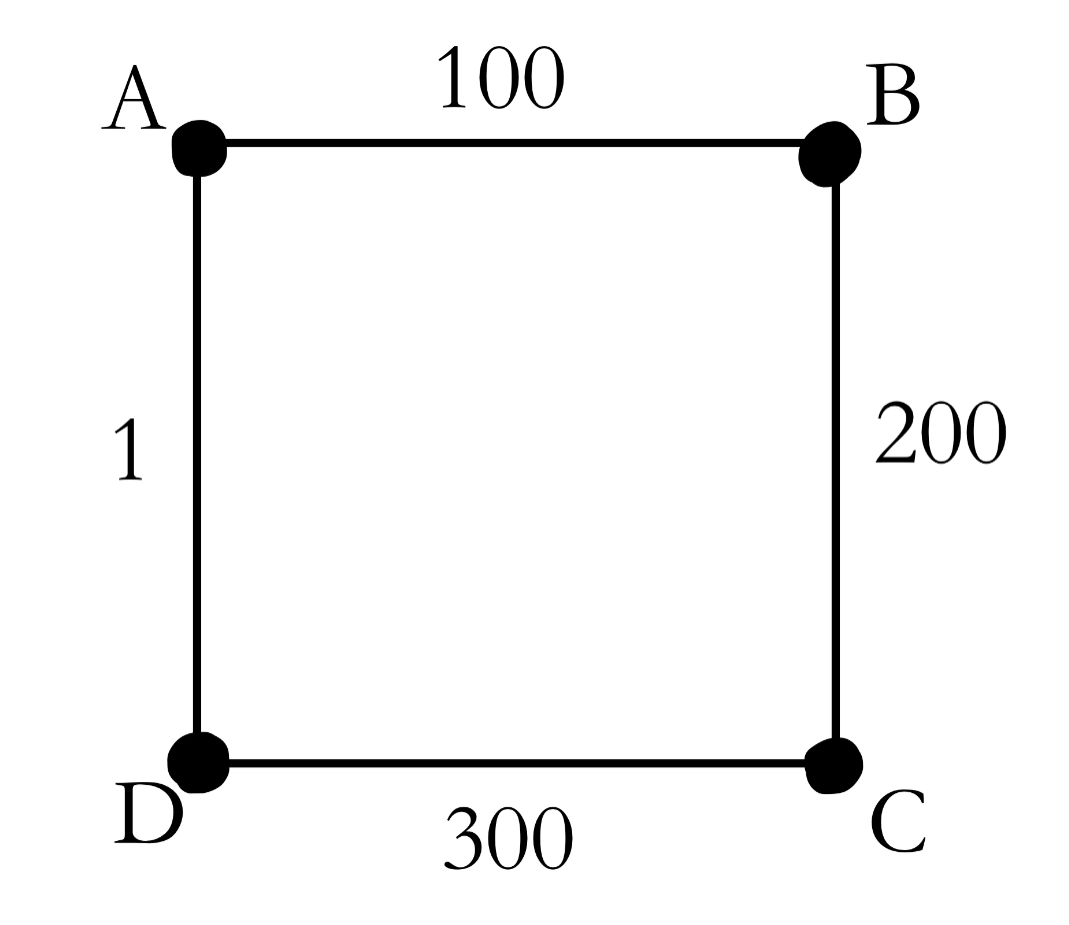
\includegraphics[width=0.5\textwidth]{image/Ch9S2_1.png}
	\caption{第一个例子}
  \label{Ch9S2_1}
\end{figure}

\subsection{满足两集合不相等的例子}

如例子二,此图\ref{Ch9S2_2}的$ max(A) = (A,B) , max(B) = (A,B) , max(C) = (C,D) , max(D) = (C,D) $,那么$ S_G = {(A,B),(C,D)} $

而此图的最大生成树显然是$ T_G = {(A,B),(B,C),(C,D)} \neq S_G$

\begin{figure}[htbp]
	\centering
	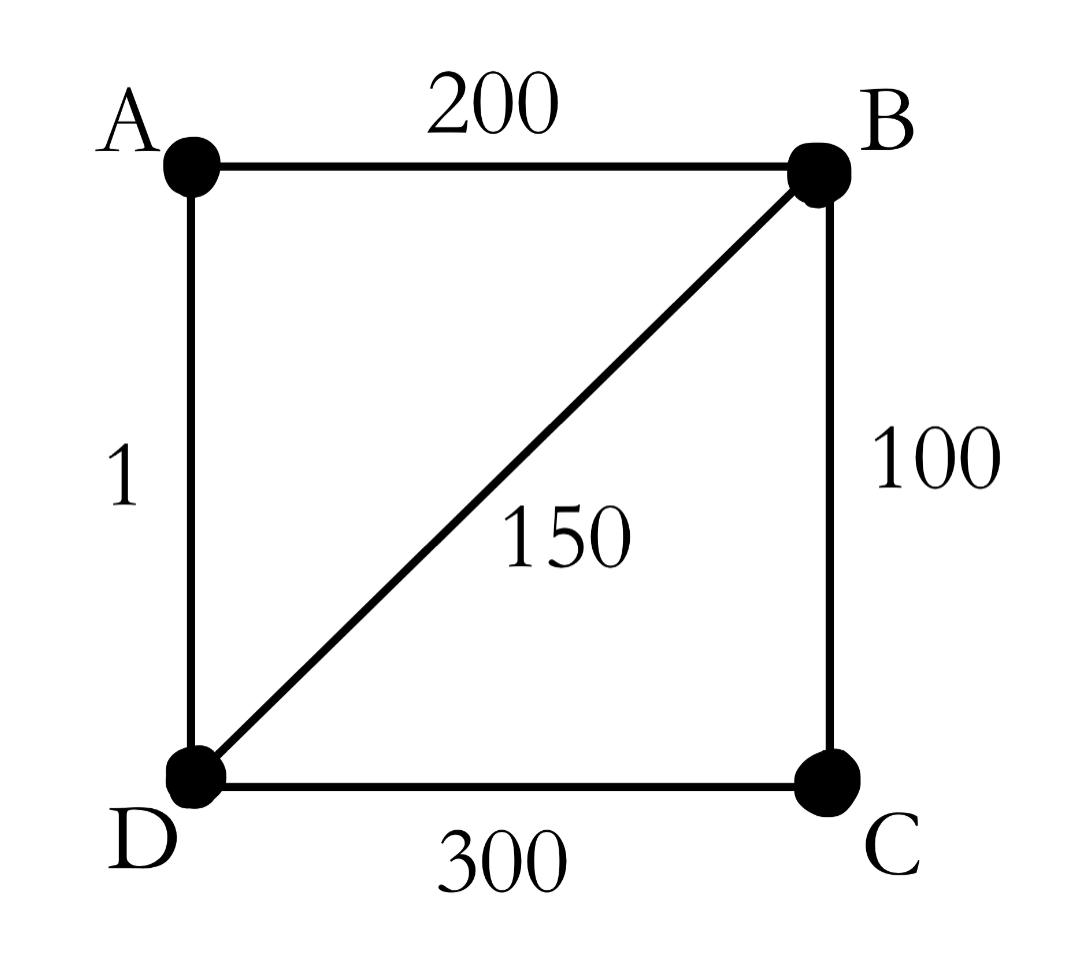
\includegraphics[width=0.5\textwidth]{image/Ch9S2_2.png}
	\caption{第二个例子}
  \label{Ch9S2_2}
\end{figure}

\subsection{证明S是T的子集}

\textbf{证明:}假设$ S_G $不是$ T_G $的子集,即$ \exists (u,v) \in S_G$但是$ (u,v) \notin T_G$,那么将$ (u,v) $加入$ T_G $得到$ T_G' $,此集合中必存在环,而且由于在增加边之前的集合是树,那么新生成的环必然包含$ (u,v) $,不然若去掉$ (u,v) $恢复到$ T_G $,环依然存在,与其为树的前提矛盾.若新生成的环不止一个,那么两个以$ (u,v) $为公共边的环在去掉$ (u,v) $还原为$ T_G $后仍然能连成环,与$ T_G $为树的前提矛盾,所以至多存在一个环,于是在环中找到权值最小的边将其删去得到$ T_G'' $,其必然无环且边数恰为顶点数$ -1 $,易证其仍然为树,显然$ \omega(T_G'') > \omega(T_G) $,这与$ T_G $是最大生成树的前提矛盾,所以假设不成立,所以$ S_G \subseteq T_G $.

\subsection{证明权重不等式}

\textbf{证明:}此处引用上一题结论,$ S_G \subseteq T_G$,假设我们以每次查找在不会成环的前提下所能加入的最大权值边的算法生成$ T_G $,其边加入的顺序应当恰好为$ T_G $中边权值从大到小的排序,模拟这个加入边的过程,若$ \exists (u,v) \in (T_G - S_G) $,在这条边刚加入集合的时候,可知$ (u,v) \neq max(u) $且$ (u,v) \neq max(v) $,而$ \omega(u,v) \le \omega(max(u)) $且$ \omega(u,v) \le \omega(max(v))$,那么由上题结论,显然$ max(u) $和$ max(v) $已经在集合中了。

所以,在$ T_G $中,$ (T_G-S_G) $的任何一条边$ u $必然被至少两条$S_G$中的边$ v1,v2 $分别紧邻两个端点,且不同的边$ u_i $所对应的$ v1_i,v2_i $不可能完全相同,又根据配对规则,$ |S_G| \ge \ulcorner |V|/2  \urcorner $,而$ |T_G| = |V| - 1 $,所以显然$ |T_G-S_G|\le \llcorner |V|/2 \lrcorner -1 < |S_G| $,将边视作“点”而绘制$ T_G $的边图,令$ X = (T_G-S_G),Y = S_G $,易证其满足Hall定理条件,于是得到必然存在一种匹配法可以将所有的$ (T_G-S_G) $中的边与$ S_G $中的一些边一一匹配,令这些被匹配的属于$ S_G $的边的集合为$ S_G' \subseteq S_G $,所以有:
\begin{equation}
	\begin{aligned}
		\omega(T_G) &= \omega(S_G) + \omega(T_G-S_G) \\
					&\le \omega(S_G) + \omega(S_G') \\
					&\le 2\omega(S_G) 
	\end{aligned}
	\nonumber
\end{equation}
所以有:
\begin{equation}
	\omega(S_G) \ge \omega(T_G)/2 \nonumber
\end{equation}

\subsection{计算2近似的最大生成树算法}

\begin{lstlisting}
APPROX-MAX-SPAN-TREE
	v = G.vexnum 
	e = G.edgenum
	let S1-Sv be any edge
	set each S1.s case to 1,mark each edge to white
	for each edge (u,v)
		if w(u,v) > w(Su)
			Su.case--
			Su = (u,v)
			(u,v).case++
			if w(u,v) > w(Sv)
				mark Sv to grey
				mark Su to grey
				Sv = (u,v)
				(u,v).case++
			else
				mark sv to white
				mark su to white
	let TSet be an empty set
	let Cross1Set be an empty set
	let Cross2Set be an empty set
	i = 1
	j = 1
	while(1)
		if Si is while
			add Si to Tset
			i = vi //Si = (ui,vi)
		else if grey
			add Si to Tset
			mark Su,Sv to black
		else
	for each edge
		if not circle && i.case == 0
			add i to Tset
\end{lstlisting}

\end{document}
